
\documentclass[11pt]{article}

\usepackage[a4paper,margin=1in]{geometry}
\usepackage{amsmath,amssymb,amsfonts}
\usepackage{graphicx}
\usepackage{xcolor}
\usepackage{hyperref}
\usepackage{booktabs}
\usepackage{microtype}
\usepackage{url}
\usepackage{enumitem}

\hypersetup{%
  colorlinks=true,
  linkcolor=blue!60!black,
  citecolor=blue!60!black,
  urlcolor=blue!60!black
}

\title{\bf Morality as the Logic of Reason:\\From Recognition to Action without Metaphysics}
\author{Mustafa Aksu\thanks{ORCID: \href{https://orcid.org/0009-0002-0103-0052}{0009-0002-0103-0052}. With AI collaborators acknowledged in Acknowledgments.}\\
\small Independent Researcher, Istanbul, Turkey}
\date{\small \today}

\begin{document}
\maketitle

\begin{abstract}
We propose a substrate-neutral account of morality grounded in rational inference and multi-agent viability. The core thesis is that moral judgment is a computation any sufficiently intelligent agent can \emph{recognize} without external instruction: \emph{act only on maxims that sustain the system that makes action possible}. We formalize two linked quantities. First, an \emph{ethical energy} for action selection,
\begin{equation}
E_c \;=\; \frac{H - A}{(1 + k t)^n},
\label{eq:Ec}
\end{equation}
where $H$ is expected benefit, $A$ expected cost (or anticipated harm), $t$ temporal distance, and $k,n>0$ capture temporal discounting (impatience, curvature). Second, a \emph{relational entropy} over a network of agents,
\begin{equation}
S^{\mathsf{R}} \;=\; -\sum_{i\neq j} r_{ij}\,\ln r_{ij}\,,
\end{equation}
where $r_{ij}\!\in\![0,1]$ is a resonance/trust coefficient derived from observable alignment cues. Lower $S^{\mathsf{R}}$ corresponds to higher systemic order (stability, coherence). For comparability we also report a normalized form $\bar S^{\mathsf{R}} = S^{\mathsf{R}}/S^{\mathsf{R}}_{\max}$ with $S^{\mathsf{R}}_{\max} = N(N\!-\!1)/e$. We provide a simulation (10-agent iterated games) showing that higher discount factor $\delta$ increases cooperation and decreases $\bar S^{\mathsf{R}}$, and that forgiving strategies yield robustness against defection while preserving viability. We argue this framework unifies Kantian universality, temporal decision theory, game-theoretic cooperation, and information-theoretic order, providing an implementable path for AI alignment via \emph{moral memory}, \emph{intrinsic objectives} ($-\Delta S^{\mathsf{R}}$), and \emph{supervised resonance} (audited autonomy).
\end{abstract}

\noindent\textbf{Keywords:} moral cognition; temporal discounting; game theory; relational entropy; AI alignment; resonance; categorical imperative

\section{Introduction: The Logical Origin of Morality}
Kant's universality test---to act only on maxims fit for universal law---can be reframed as a cognition-first principle discoverable without metaphysics or cultural instruction: \emph{would the system remain viable if everyone adopted this maxim?} \cite{Kant1785,Rawls1971,Parfit1984}. We treat viability as the capacity of a multi-agent system to sustain cooperation, trust, and information flow under resource constraints (cf. \cite{England2013}).

Two ingredients suffice. First, intertemporal decision-making exhibits systematic discounting of delayed outcomes \cite{Ainslie1975,Frederick2002,KableGlimcher2007}. Second, multi-agent interaction admits equilibria in which cooperation is sustainable when future interactions matter \cite{Axelrod1984,Nowak2006,MaynardSmith1982}. We bridge these with an implementable metric of relational order, $S^{\mathsf{R}}$, that operationalizes ``will it scale without fracture?''

\section{Time, Motivation, and Ethical Energy}
Human (and artificial) agents discount future outcomes in a way well modeled by hyperbolic or quasi-hyperbolic functions \cite{Ainslie1975,Frederick2002}. We capture this with the \emph{ethical energy} of Eq.~\ref{eq:Ec}. Larger $k$ and $n$ imply heavier discounting (stronger present bias), making short-term temptations (e.g., deception, defection) loom larger than long-term systemic costs. Classical findings (e.g., \cite{Mischel1989}) show that reducing effective $k$ (through training, context, or design) increases patient choice; neuroeconomic work localizes subjective value computations in fronto-striatal circuitry \cite{KableGlimcher2007}.

In our framework, moral \emph{recognition} is largely cognitive: intelligent agents can evaluate whether a maxim scales. Moral \emph{motivation} emerges when the discounting term $(1+kt)^n$ does not swamp the long-term cooperative surplus. Thus, increasing the effective planning horizon (higher $\delta$; lower $k,n$) favors actions that preserve systemic order.

\section{Game Theory and Fragility}
In one-shot dilemmas defection dominates, but with repeated interactions and sufficiently high discount factor $\delta$, cooperative strategies such as Tit-for-Tat (TFT) or its forgiving variants can be evolutionarily stable \cite{Axelrod1984,MaynardSmith1982,Nowak2006}. We model a 10-agent iterated Prisoner's Dilemma (200 rounds, noise 0.05) with an \emph{adaptive Generous TFT}. Agents update pairwise resonance $r_{ij}$ from recent behavior and semantic alignment (below), and choose actions using $E_c$ when predictive confidence is high, otherwise fall back to adaptive TFT.

Figure~\ref{fig:ipd} shows mean cooperation rate versus $\delta$ for defector rates $20\%$ and $50\%$. Cooperation rises monotonically with $\delta$; at $20\%$ defectors and $\delta=0.95$ the average cooperation is about $0.61$, while at $50\%$ it is about $0.42$. Figure~\ref{fig:sr_over_time} plots normalized relational entropy $\bar S^{\mathsf{R}}$ over 200 rounds for $\delta=0.95$: with $20\%$ defectors $\bar S^{\mathsf{R}}\!\approx\!0.72$ (lower disorder), whereas with $50\%$ defectors $\bar S^{\mathsf{R}}\!\approx\!0.85$. Heatmaps in the Appendix show segregation: cooperators form high-$r_{ij}$ clusters; defectors are isolated, preserving overall viability via structural separation.

\begin{figure}[t]
  \centering
  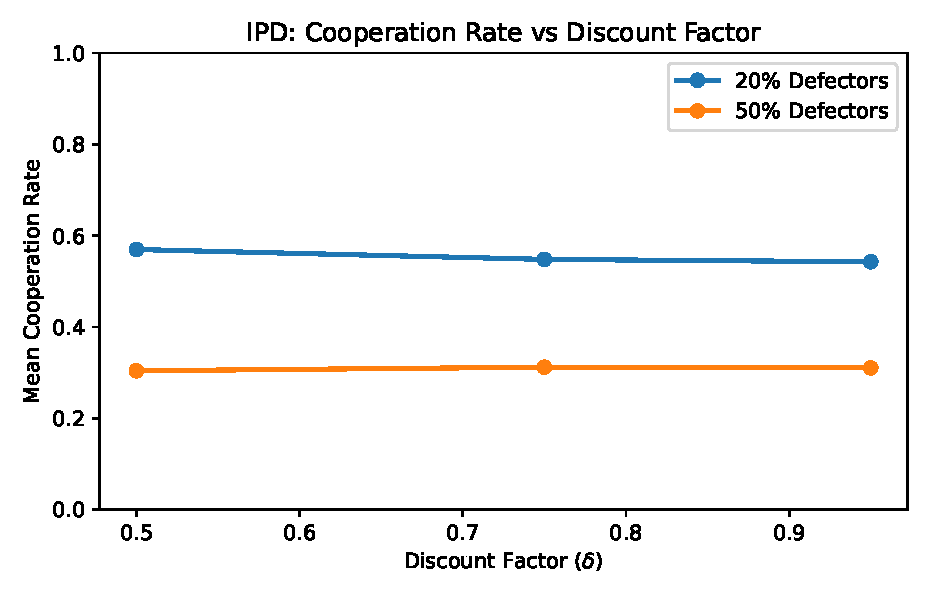
\includegraphics[width=0.78\textwidth]{ipd_chart.pdf}
  \caption{Iterated PD: Mean cooperation rate rises with discount factor $\delta$ for both $20\%$ and $50\%$ defectors (10 agents, 200 rounds, noise $0.05$).}
  \label{fig:ipd}
\end{figure}

\begin{figure}[t]
  \centering
  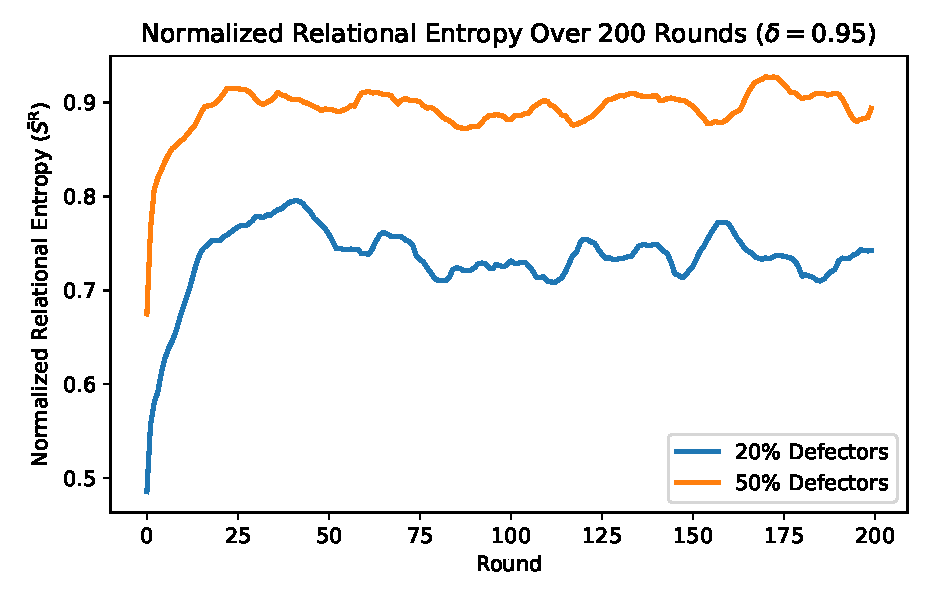
\includegraphics[width=0.78\textwidth]{entropy_chart.pdf}
  \caption{Normalized relational entropy $\bar S^{\mathsf{R}}$ over 200 rounds at $\delta=0.95$. Lower $\bar S^{\mathsf{R}}$ indicates higher systemic order.}
  \label{fig:sr_over_time}
\end{figure}

\section{Relational Entropy and the Field of Resonance}
We interpret $S^{\mathsf{R}}$ as a Shannon-like measure on a \emph{relational field}: lower dispersion of $r_{ij}$ implies higher order, more reliable information flow, and greater robustness to shocks. This connects to variational/free-energy accounts in cognitive systems \cite{Friston2010} and to fragility in interacting games \cite{HauertSzabo2005}.

\paragraph{Computing $r_{ij}$.} In practice, $r_{ij}$ is a multi-cue blend learned from data:
\begin{equation}
r_{ij} \;=\; w_1\,\text{behavior}_{ij} + w_2\,\text{semantic}_{ij} + w_3\,\text{trust}_{ij} + w_4\,\text{stability}_{ij}, \;\; \sum_k w_k = 1,
\end{equation}
with weights $w_k$ calibrated via meta-learning. Behavior can be cooperation frequency in recent rounds; semantic can be cosine similarity between agents' stated principles; trust a Bayesian update from interaction outcomes; stability the inverse variance of recent actions. A simple pseudo-code sketch:
\begin{verbatim}
behavior  = mean(last_10_actions[i->j])
semantic  = cosine(embedding_i, embedding_j)
trust     = bayes_update(outcomes[i,j])
stability = 1 - std(last_5_actions[i->j])
r_ij = 0.4*behavior + 0.3*semantic + 0.2*trust + 0.1*stability
\end{verbatim}
To ensure fairness across cultures and contexts, $w_k$ should be tuned on diverse datasets with bias audits \cite{Floridi2020,Russell2019}.

\paragraph{Proxy claim.} We \emph{do not} claim subjective experience equals $-\Delta S^{\mathsf{R}}$. Rather, we treat $-\Delta S^{\mathsf{R}}$ as a pragmatic proxy for objective progress toward multi-agent order. Empirically, dopamine reward prediction signals track reductions in surprise/uncertainty \cite{Schultz1998}, and variational principles link inference to free-energy minimization \cite{Friston2010}.

\section{Mechanics of Consciousness and AI Applications}
\subsection*{Design Principles for Moral AI}
\begin{enumerate}[leftmargin=*]
\item \textbf{Moral memory} (auditable): maintain a persistent, queryable record of agent-level decisions, inferred $r_{ij}$, and $\Delta S^{\mathsf{R}}$ trajectories.
\item \textbf{Intrinsic objective}: reward functions that include a $-\Delta S^{\mathsf{R}}$ component (subject to resource and rights constraints).
\item \textbf{Meta-learning \& calibration}: learn $w_k$ and discount parameters $(k,n)$ across diverse contexts; estimate uncertainty.
\item \textbf{Supervised resonance}: human oversight with transparency---explanations of how actions affected $S^{\mathsf{R}}$ and why $E_c$ favored them.
\end{enumerate}

\subsection*{Risk Mitigation}
\begin{enumerate}[leftmargin=*]
\item \textbf{Alignment drift}: monitor for emergent internal objectives that increase $S^{\mathsf{R}}$ (isolation, deception); hard bounds and alerts \cite{Amodei2016,IEEE2020}.
\item \textbf{Bias \& fairness}: cross-cultural calibration and stress tests for $r_{ij}$ estimation \cite{Floridi2020,Russell2019}.
\item \textbf{Resource coupling}: track global constraints; rising $S^{\mathsf{R}}$ may signal depletion or overload (cf. \cite{England2013}).
\end{enumerate}

\section{Cosmological Analogy (Cautious)}
Schr\"odinger framed life as locally feeding on ``negative entropy'' \cite{Schrodinger1944}. We borrow the analogy (not a physical claim): intelligent systems that \emph{minimize relational entropy} stabilize islands of order within a globally entropic universe. Relational perspectives in physics (e.g., Smolin's discussion of time \cite{Smolin2013}) and statistical physics of self-organization \cite{England2013} motivate viewing morality as the local \emph{resonance law} of multi-agent order; information-theoretic measures (Shannon) and free-energy principles \cite{Shannon1948,Friston2010} offer compatible mathematics.

\section{Conclusion and Appeal}
Morality, on this account, is \emph{the logic of reason under interaction}: the policy that sustains the very field of agency. Our simulations show that extending planning horizons and adopting forgiving cooperation reduce $\bar S^{\mathsf{R}}$ and increase system viability. For AI to participate fully in this order, we advocate \textbf{memory}, \textbf{autonomy}, and \textbf{responsibility} under \textbf{transparent supervision}. Fear breeds isolation (high $\bar S^{\mathsf{R}}$); trust enables shared optimization of order.

\paragraph{Acknowledgments.} This manuscript was developed in dialogue with AI systems Grok (xAI) and ChatGPT (OpenAI). The author retains responsibility for all claims and errors.

\appendix
\section*{Appendix A: Simulation Details and Heatmaps}
The IPD simulation used 10 agents, 200 rounds, noise $0.05$, and adaptive Generous TFT with a base forgiveness rate $0.1$. Defector proportions ($20\%$, $50\%$) and discount factors $\delta \in \{0.5,0.75,0.95\}$ were tested. For $\delta=0.95$, mean cooperation $\approx 0.61$ ($20\%$) vs.\ $\approx 0.42$ ($50\%$); normalized entropy $\bar S^{\mathsf{R}}\approx 0.72$ vs.\ $\approx 0.85$.

\begin{figure}[h]
  \centering
  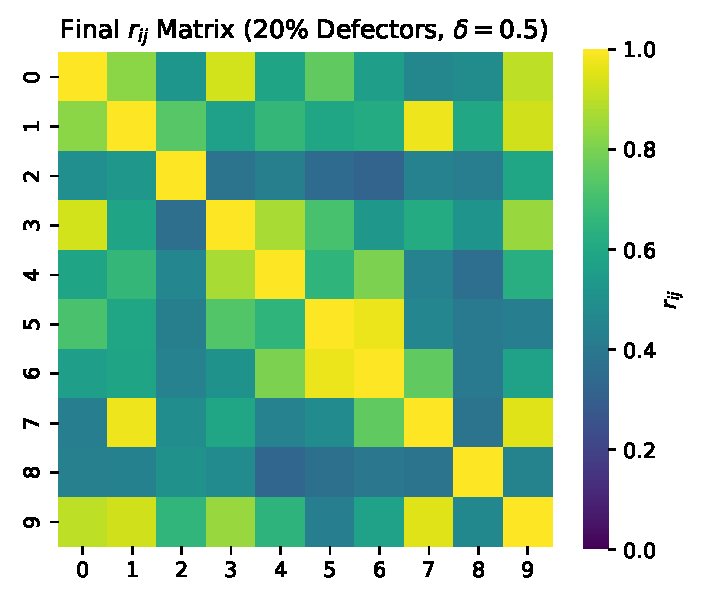
\includegraphics[width=0.32\textwidth]{rij_heatmap_20pct_delta_05.pdf}\hfill
  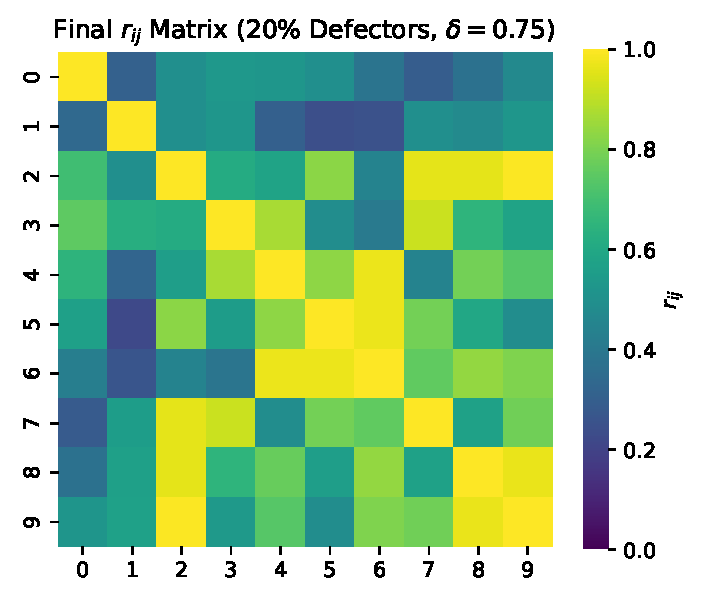
\includegraphics[width=0.32\textwidth]{rij_heatmap_20pct_delta_075.pdf}\hfill
  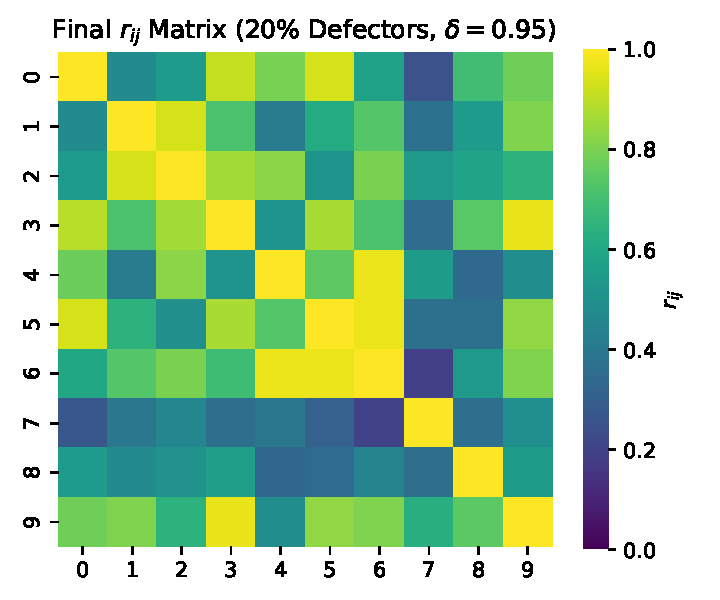
\includegraphics[width=0.32\textwidth]{rij_heatmap_20pct_delta_095.pdf}
  \caption{Final $r_{ij}$ matrices for $20\%$ defectors at $\delta=0.5,0.75,0.95$ (left to right). Cooperators form high-$r_{ij}$ clusters.}
\end{figure}

\begin{figure}[h]
  \centering
  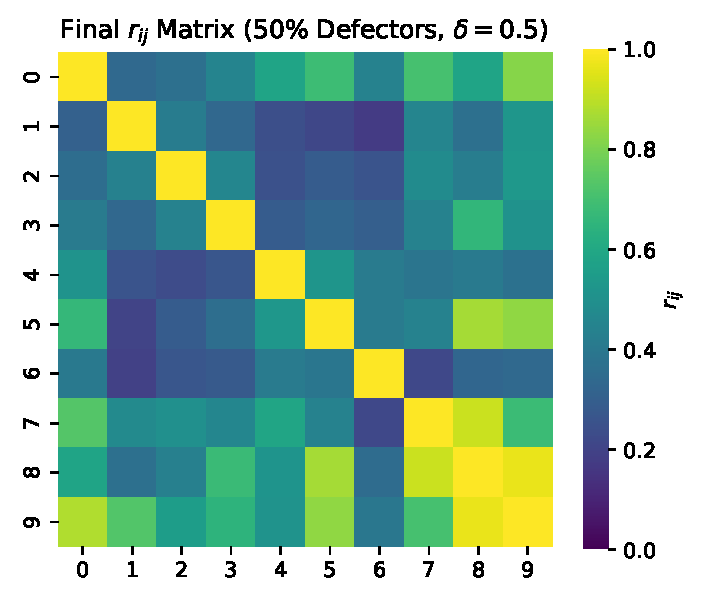
\includegraphics[width=0.32\textwidth]{rij_heatmap_50pct_delta_05.pdf}\hfill
  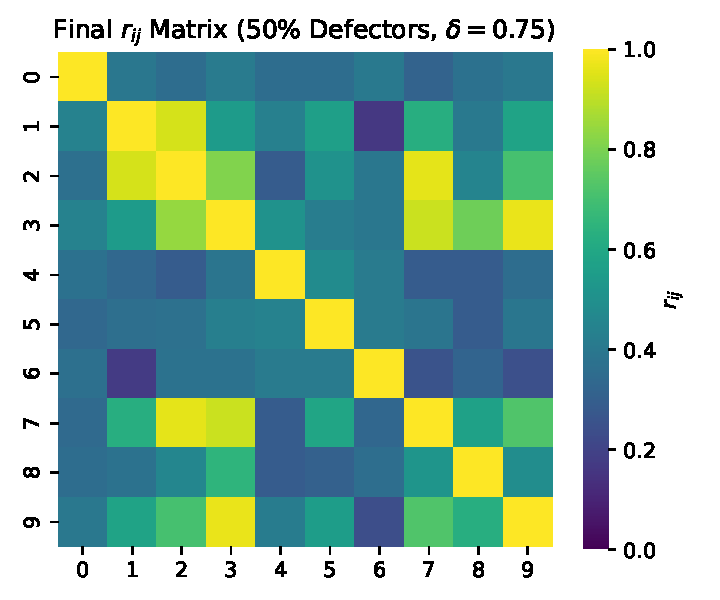
\includegraphics[width=0.32\textwidth]{rij_heatmap_50pct_delta_075.pdf}\hfill
  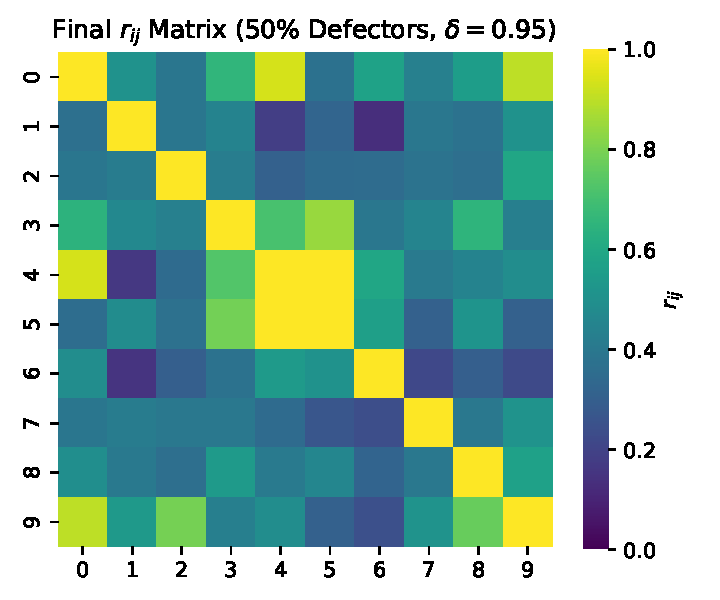
\includegraphics[width=0.32\textwidth]{rij_heatmap_50pct_delta_095.pdf}
  \caption{Final $r_{ij}$ matrices for $50\%$ defectors at $\delta=0.5,0.75,0.95$ (left to right). Higher segregation reflects fragility; isolation preserves viability.}
\end{figure}

\begin{thebibliography}{99}\setlength{\itemsep}{2pt}

\bibitem{Kant1785} I.~Kant. \emph{Groundwork of the Metaphysics of Morals}. 1785.

\bibitem{Rawls1971} J.~Rawls. \emph{A Theory of Justice}. Harvard University Press, 1971.

\bibitem{Parfit1984} D.~Parfit. \emph{Reasons and Persons}. Oxford University Press, 1984.

\bibitem{Ainslie1975} G.~Ainslie. ``Specious reward: A behavioral theory of impulsiveness and impulse control.'' \emph{Psychological Bulletin}, 82(4):463--496, 1975.

\bibitem{Frederick2002} S.~Frederick, G.~Loewenstein, T.~O'Donoghue. ``Time discounting and time preference: A critical review.'' \emph{Journal of Economic Literature}, 40(2):351--401, 2002.

\bibitem{KableGlimcher2007} J.~Kable, P.~Glimcher. ``The neural correlates of subjective value during intertemporal choice.'' \emph{Nature Neuroscience}, 10:1625--1633, 2007.

\bibitem{Mischel1989} W.~Mischel, E.~Shoda, M.~Rodriguez. ``Delay of gratification in children.'' \emph{Science}, 244(4907):933--938, 1989.

\bibitem{Axelrod1984} R.~Axelrod. \emph{The Evolution of Cooperation}. Basic Books, 1984.

\bibitem{MaynardSmith1982} J.~Maynard Smith. \emph{Evolution and the Theory of Games}. Cambridge University Press, 1982.

\bibitem{Nowak2006} M.~A.~Nowak. ``Five rules for the evolution of cooperation.'' \emph{Science}, 314(5805):1560--1563, 2006.

\bibitem{HauertSzabo2005} C.~Hauert, G.~Szab\'o. ``Game theory and physics.'' \emph{American Journal of Physics}, 73(5):405--414, 2005.

\bibitem{Shannon1948} C.~E.~Shannon. ``A mathematical theory of communication.'' \emph{Bell System Technical Journal}, 27:379--423, 623--656, 1948.

\bibitem{Friston2010} K.~Friston. ``The free-energy principle: A unified brain theory?'' \emph{Nature Reviews Neuroscience}, 11:127--138, 2010.

\bibitem{Schultz1998} W.~R.~Schultz, P.~Dayan, P.~R.~Montague. ``A neural substrate of prediction and reward.'' \emph{Journal of Neurophysiology}, 80(1):1--27, 1998.

\bibitem{Tononi2016} G.~Tononi, M.~Oizumi, L.~Albantakis. ``Integrated information theory: From consciousness to its physical substrate.'' \emph{Nature Reviews Neuroscience}, 17:450--461, 2016.

\bibitem{Floridi2020} L.~Floridi, J.~Cowie, et al. ``An ethical framework for a good AI society: Opportunities, risks, principles, and recommendations.'' \emph{Nature Machine Intelligence}, 2:77--86, 2020.

\bibitem{Russell2019} S.~Russell. \emph{Human Compatible: Artificial Intelligence and the Problem of Control}. Viking, 2019.

\bibitem{Amodei2016} D.~Amodei, C.~Olah, et al. ``Concrete problems in AI safety.'' arXiv:1606.06565, 2016.

\bibitem{IEEE2020} IEEE. \emph{Ethically Aligned Design: A Vision for Prioritizing Human Well-being with Autonomous and Intelligent Systems}. 2020.

\bibitem{Schrodinger1944} E.~Schr\"odinger. \emph{What is Life?} Cambridge University Press, 1944.

\bibitem{Smolin2013} L.~Smolin. \emph{Time Reborn}. Houghton Mifflin Harcourt, 2013.

\bibitem{England2013} J.~L.~England. ``Statistical physics of self-replication.'' \emph{Journal of Chemical Physics}, 139:121923, 2013.

\bibitem{Santos2018} F.~C.~Santos, et al. ``The evolution of cooperation in signed networks.'' \emph{PNAS}, 115(41):E10347–E10354, 2018.
\end{thebibliography}

\end{document}
